% MORPH — Embeddings (Hybrid input representation + per-layer Bigram injection).
% The zoom-in of the "Hybrid Embedding" box in morph_overview.tex / morph_deploy_stack.tex.
% LAYOUT: left->right fan-in. Token IDs fan into the Euclidean table (top) and the
% Lorentz geometric pipeline (bottom); they concat into the hybrid input vector that
% feeds the residual stream. A separate bottom lane is the position-invariant bigram
% hash signal injected additively at every block. The LM head is weight-tied to the
% Euclidean+Lorentz-tangent weights (drawn as a dashed weight-tie, not a data arrow).
%
% Verified against code (2026-06-07, morph/model/embeddings.py + embed_quant.py + transformer.py):
%   - HybridEmbedding.forward = cat([euc_embed(ids) [V,d_e] || lorentz_tangent(ids) [V,d_L]]),
%     computed ONCE; d_e = d_model - d_L; lorentz_fraction=0.25 -> d_e=576, d_L=192 at d=768.
%   - Lorentz: space_embed -> project_to_hyperboloid (x0=sqrt(1+||xs||^2)) -> log_map_origin
%     (drop x0, scale acosh(x0)/sqrt(x0^2-1)) -> d_L tangent vector. Init std 0.005.
%   - Bigram: key=(A*id_t XOR B*id_{t-1}) mod 49152 (A=279470273,B=4294967291); table [49152,d];
%     inject x + lambda_layer*bigram at EVERY block; per-layer lambda init 0 (learned).
%   - LM head: lm_weight = cat([euc_w || lorentz_tangent_w]); logits = h @ W^T, cast fp32 (fused_ce).
%   - Quant (Ablation E, embed_quant.py): per-row absmax int-N STE (s_row=max|w_row|/hi) on
%     euc_embed + bigram.embed ONLY. Lorentz space_embed ALWAYS bf16 (safety-guarded, raises if
%     touched). lm_head_quant = NO-OP at weight level (head tied to euc_embed); logits fp32.
% Compile: pdflatex morph_embeddings.tex
%
% NOTE: base.yaml uses embed_quant="int6" for Euclidean and bigram rows. The Lorentz
% embedding remains bf16 and is guarded against quantization in embed_quant.py.

\documentclass[border=14pt]{standalone}
\usepackage[T1]{fontenc}
\usepackage{amsmath,amssymb}
\usepackage{tikz}
\usetikzlibrary{arrows.meta, fit, positioning, calc, backgrounds, decorations.pathreplacing}

% ── Palette (Paul Tol, colorblind-safe — matches the figure family) ───────────
\definecolor{cbBlue}{HTML}{4477AA}
\definecolor{cbOrange}{HTML}{EE7733}
\definecolor{cbPurple}{HTML}{AA3377}
\definecolor{cbTeal}{HTML}{228833}
\definecolor{cbGray}{HTML}{777777}
\definecolor{fBlue}{HTML}{DCEAF7}
\definecolor{fOrange}{HTML}{FDE8D0}
\definecolor{fPurple}{HTML}{EEDCEE}
\definecolor{fTeal}{HTML}{D6EFDD}
\definecolor{fGray}{HTML}{EBEBEB}
\definecolor{bdr}{HTML}{555555}

% ── Precision palette (identical to morph_deploy_stack.tex) ───────────────────
\definecolor{pBf16}{HTML}{08519C}   % deep blue  — bf16 (Lorentz, geometry-sensitive)
\definecolor{pInt6}{HTML}{009E73}   % green      — int6 (euclidean + bigram tables)

\tikzset{
  io/.style={font=\small\sffamily},
  % generic box
  EB/.style={draw=bdr, thick, rounded corners=4pt, minimum width=3.4cm,
    minimum height=1.15cm, font=\scriptsize\sffamily, align=center, inner sep=4pt},
  % precision-colored boxes (border = precision; text badge is authoritative)
  PI6/.style={EB, draw=pInt6, line width=1pt, fill=pInt6!14},   % int6 (green)
  PB/.style={EB, draw=pBf16, line width=1pt, fill=pBf16!12},    % bf16 (deep blue)
  proc/.style={EB, draw=pBf16!80!black, line width=0.8pt, fill=pBf16!5},  % bf16 geometry op (no params)
  neutral/.style={EB, draw=bdr, fill=fGray!35},
  ghash/.style={EB, draw=cbGray, line width=0.8pt, fill=fGray!45},
  % precision badge (text spelled out — never color-only)
  badge/.style={draw=#1, line width=1pt, rounded corners=3pt, fill=#1!18,
    font=\scriptsize\sffamily\bfseries, text=#1!60!black, inner sep=3pt,
    align=center, minimum height=0.5cm},
  A/.style={-{Stealth[length=2.8mm,width=2.2mm]}, thick},
  As/.style={-{Stealth[length=2.4mm,width=1.9mm]}, semithick},
  Ad/.style={-{Stealth[length=2.4mm,width=1.9mm]}, thick, densely dashed},
  sub/.style={font=\scriptsize\sffamily},
  tny/.style={font=\tiny\sffamily},
  dim/.style={font=\tiny\sffamily, text=cbGray},
}

\begin{document}
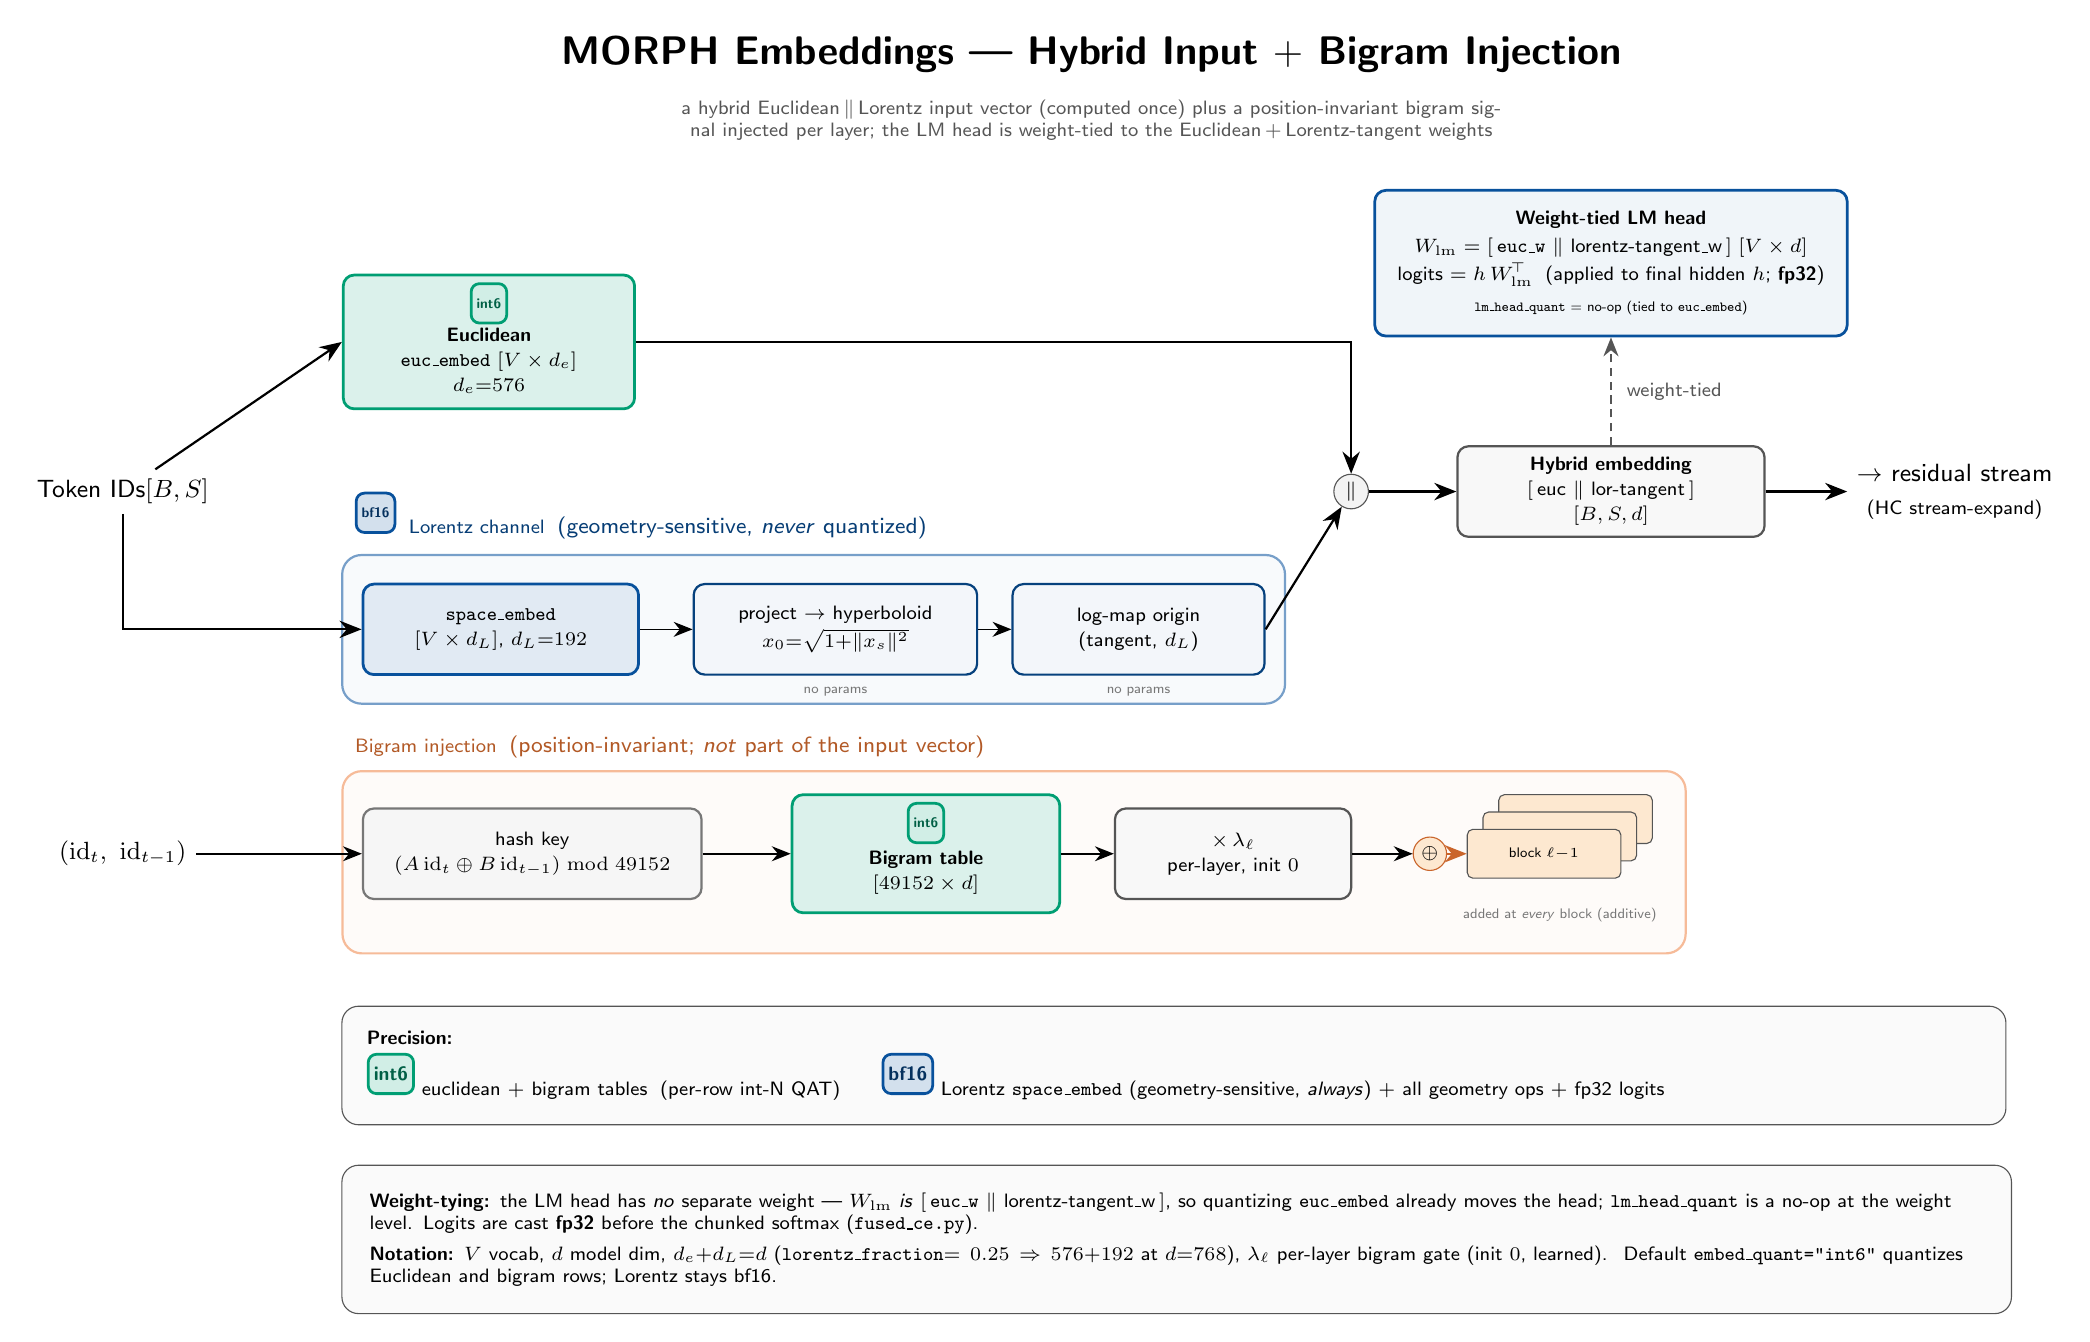
\begin{tikzpicture}

% =====================================================================
% BAND A — Hybrid input representation (computed once)
% =====================================================================
\node[io] (tok) at (-13.9,2.75) {Token IDs\\[1pt]$[B,S]$};

% Euclidean channel (top, int6)
\node[PI6, minimum width=3.7cm, minimum height=1.7cm] (euc) at (-9.25,4.65) {%
  \rule{0pt}{0.44cm}\\[-2pt]
  \textbf{Euclidean}\\[1pt]\texttt{euc\_embed} $[V\times d_e]$\\[1pt]$d_e{=}576$};
\node[badge=pInt6, anchor=north, inner sep=2pt, font=\tiny\sffamily\bfseries]
  at ($(euc.north)+(0,-0.11)$) {int6};

% Lorentz channel (bottom strip, all bf16)
\node[PB, minimum width=3.5cm] (lspace) at (-9.1,1.0) {%
  \texttt{space\_embed}\\[1pt]$[V\times d_L]$, $d_L{=}192$};
\node[proc, minimum width=3.6cm] (lhyp) at (-4.85,1.0) {%
  project $\to$ hyperboloid\\[1pt]$x_0{=}\sqrt{1{+}\lVert x_s\rVert^2}$};
\node[proc, minimum width=3.2cm] (llog) at (-1.0,1.0) {%
  log-map origin\\[1pt](tangent, $d_L$)};
\foreach \a/\b in {lspace/lhyp, lhyp/llog}{\draw[As] (\a)--(\b);}
\node[dim, anchor=north] at ($(lhyp.south)+(0,-0.02)$) {no params};
\node[dim, anchor=north] at ($(llog.south)+(0,-0.02)$) {no params};
% Lorentz container
\begin{scope}[on background layer]
  \node[draw=pBf16!55, thick, rounded corners=7pt, fill=pBf16!3,
        fit=(lspace)(llog), inner xsep=7pt, inner ysep=10pt] (LBOX) {};
\end{scope}
\node[sub, text=pBf16!75!black, anchor=south west] at ($(LBOX.north west)+(0.05,0.06)$)
  {\tikz\node[badge=pBf16, inner sep=2pt, font=\tiny\sffamily\bfseries]{bf16};\; Lorentz channel \;{\footnotesize(geometry-sensitive, \emph{never} quantized)}};

% Token IDs fan out into both channels
\draw[A] (tok) -- (euc.west);
\draw[A] (tok) |- (lspace.west);

% Concat -> hybrid vector
\node[circle, draw=bdr, fill=fGray!60, inner sep=1.6pt,
      font=\scriptsize\sffamily] (cat) at (1.7,2.75) {$\Vert$};
\node[neutral, minimum width=3.9cm] (hyb) at (5.0,2.75) {%
  \textbf{Hybrid embedding}\\[1pt]$[\,$euc $\Vert$ lor-tangent$\,]$\\[1pt]$[B,S,d]$};
\draw[A] (euc.east) -| (cat);
\draw[A] (llog.east) -- (cat);
\draw[A] (cat) -- (hyb);
\node[io, align=center, anchor=west] (resid) at (8.0,2.75)
  {$\to$ residual stream\\[1pt]{\scriptsize(HC stream-expand)}};
\draw[A] (hyb) -- (resid);

% =====================================================================
% Weight-tied LM head (full) — dashed weight-tie, NOT a data-flow arrow
% =====================================================================
\node[PB, minimum width=6.0cm, minimum height=1.85cm, fill=pBf16!6] (lm) at (5.0,5.65) {%
  \textbf{Weight-tied LM head}\\[2pt]
  {\scriptsize $W_\mathrm{lm}=[\,$\texttt{euc\_w} $\Vert$ lorentz-tangent\_w$\,]\;[V\times d]$}\\[1pt]
  {\scriptsize logits $= h\,W_\mathrm{lm}^{\!\top}$ \;(applied to final hidden $h$; \textbf{fp32})}\\[3pt]
  {\tiny\texttt{lm\_head\_quant} = no-op (tied to \texttt{euc\_embed})}};
\draw[Ad, bdr] (hyb.north) -- (lm.south)
  node[pos=0.5, right=2pt, sub, text=bdr]{weight-tied};

% =====================================================================
% BAND B — Bigram injection (per-layer additive, position-invariant)
% =====================================================================
\def\by{-1.85}
\node[io] (bg) at (-13.9,\by) {$(\mathrm{id}_t,\ \mathrm{id}_{t-1})$};
\node[ghash, minimum width=4.3cm] (hash) at (-8.7,\by) {%
  hash key\\[1pt]$(A\,\mathrm{id}_t \oplus B\,\mathrm{id}_{t-1})\bmod 49152$};
\node[PI6, minimum width=3.4cm, minimum height=1.5cm] (btab) at (-3.7,\by) {%
  \rule{0pt}{0.44cm}\\[-2pt]
  \textbf{Bigram table}\\[1pt]$[49152\times d]$};
\node[badge=pInt6, anchor=north, inner sep=2pt, font=\tiny\sffamily\bfseries]
  at ($(btab.north)+(0,-0.11)$) {int6};
\node[neutral, minimum width=3.0cm] (lam) at (0.2,\by) {%
  $\times\,\lambda_\ell$\\[1pt]{\scriptsize per-layer, init $0$}};
\foreach \a/\b in {bg/hash, hash/btab, btab/lam}{\draw[As] (\a)--(\b);}

% injection motif: added into the residual at every block
\node[draw=bdr, rounded corners=2pt, fill=fOrange, minimum width=1.95cm,
      minimum height=0.62cm, font=\tiny\sffamily] (blk3) at (4.55,\by+0.44) {block $\ell{+}1$};
\node[draw=bdr, rounded corners=2pt, fill=fOrange, minimum width=1.95cm,
      minimum height=0.62cm, font=\tiny\sffamily] (blk2) at (4.35,\by+0.22) {block $\ell$};
\node[draw=bdr, rounded corners=2pt, fill=fOrange, minimum width=1.95cm,
      minimum height=0.62cm, font=\tiny\sffamily] (blk1) at (4.15,\by) {block $\ell{-}1$};
\node[circle, draw=cbOrange!85!black, fill=fOrange, inner sep=1.4pt,
      font=\scriptsize\sffamily] (inj) at (2.7,\by) {$\oplus$};
\draw[As] (lam) -- (inj);
\draw[A, cbOrange!85!black] (inj) -- (blk1.west);
\node[dim, anchor=north, align=center] (bcap) at (4.35,\by-0.56)
  {added at \emph{every} block (additive)};

% Bigram lane container
\begin{scope}[on background layer]
  \node[draw=cbOrange!50, thick, rounded corners=7pt, fill=cbOrange!3,
        fit=(hash)(btab)(lam)(inj)(blk1)(blk3)(bcap), inner xsep=7pt, inner ysep=8pt] (BGBOX) {};
\end{scope}
\node[sub, text=cbOrange!75!black, anchor=south west] at ($(BGBOX.north west)+(0.05,0.03)$)
  {Bigram injection \;{\footnotesize(position-invariant; \emph{not} part of the input vector)}};

% =====================================================================
% Precision legend (matches morph_deploy_stack.tex)
% =====================================================================
\node[draw=bdr, rounded corners=6pt, fill=fGray!25, inner sep=9pt,
      align=left, font=\scriptsize\sffamily, text width=20.5cm, anchor=north west]
      (leg) at ($(BGBOX.south west)+(0,-0.65)$) {%
  \textbf{Precision:}\\[2pt]
  \tikz\node[badge=pInt6, inner sep=2pt]{int6};~euclidean $+$ bigram tables \;(per-row int-N QAT)\qquad
  \tikz\node[badge=pBf16, inner sep=2pt]{bf16};~Lorentz \texttt{space\_embed} (geometry-sensitive, \emph{always}) $+$ all geometry ops $+$ fp32 logits};

% =====================================================================
% Facts panel — only what the picture can't show
% =====================================================================
\node[draw=bdr, rounded corners=6pt, fill=fGray!25, inner sep=10pt,
      align=left, font=\scriptsize\sffamily, text width=20.5cm, anchor=north west]
      (facts) at ($(leg.south west)+(0,-0.5)$) {%
  \textbf{Weight-tying:} the LM head has \emph{no} separate weight — $W_\mathrm{lm}$ \emph{is} $[\,$\texttt{euc\_w} $\Vert$ lorentz-tangent\_w$\,]$,
  so quantizing \texttt{euc\_embed} already moves the head; \texttt{lm\_head\_quant} is a no-op at the weight level. Logits are cast \textbf{fp32} before the chunked softmax (\texttt{fused\_ce.py}).\\[3pt]
  \textbf{Notation:} $V$ vocab, $d$ model dim, $d_e{+}d_L{=}d$ (\texttt{lorentz\_fraction}$=0.25\Rightarrow 576{+}192$ at $d{=}768$), $\lambda_\ell$ per-layer bigram gate (init $0$, learned).
  \;Default \texttt{embed\_quant="int6"} quantizes Euclidean and bigram rows; Lorentz stays bf16.};

% =====================================================================
% Title
% =====================================================================
\node[font=\Large\sffamily\bfseries, anchor=south] (ttl) at (-1.6,7.95)
  {MORPH Embeddings --- Hybrid Input $+$ Bigram Injection};
\node[sub, text=bdr, anchor=north, below=0.1cm of ttl, text width=19cm, align=center]
  {a hybrid Euclidean\,$\Vert$\,Lorentz input vector (computed once) plus a position-invariant bigram signal injected per layer; the LM head is weight-tied to the Euclidean\,$+$\,Lorentz-tangent weights};

\end{tikzpicture}
\end{document}
